% !TeX TXS-program:compile = txs:///arara
% arara: lualatex: {shell: no, synctex: yes, interaction: batchmode}
% arara: pythontex: {rerun: modified} if found('pytxcode', 'PYTHONTEX#py')
% arara: lualatex: {shell: no, synctex: yes, interaction: batchmode} if found('pytxcode', 'PYTHONTEX#py')
% arara: lualatex: {shell: no, synctex: yes, interaction: batchmode} if found('log', '(undefined references|Please rerun|Rerun to get)')

\documentclass[a4paper,11pt]{article}
\usepackage[]{cp-base}
\graphicspath{{./graphics/}}
%variables
\donnees[%
	classe=1\up{ère} 2M2,
	matiere={[SPÉ.MATHS]},
	typedoc=CHAPITRE~,
	numdoc=13,
	titre={Fonction exponentielle}
	]

%formatage
\author{Pierquet}
\title{\nomfichier}
\hypersetup{pdfauthor={Pierquet},pdftitle={\nomfichier},allbordercolors=white,pdfborder=0 0 0,pdfstartview=FitH}
%divers
\lhead{\entete{\matiere}}
\chead{\entete{\lycee}}
\rhead{\entete{\classe{} - Chapitre \thepart}}
\lfoot{\pied{\matiere}}
\cfoot{\logolycee{}}
\rfoot{\pied{\numeropagetot}}

\tikzset{tangent/.style={% https://tex.stackexchange.com/a/25940
		decoration={%
			markings,mark=at position #1 with{
				\coordinate (tangent point-\pgfkeysvalueof{/pgf/decoration/mark info/sequence number}) at (0pt,0pt);
				\coordinate (tangent unit vector-\pgfkeysvalueof{/pgf/decoration/mark info/sequence number}) at (1,0pt);
				\coordinate (tangent orthogonal unit vector-\pgfkeysvalueof{/pgf/decoration/mark info/sequence number}) at (0pt,1);}
		},
		postaction=decorate},
	use tangent/.style={shift=(tangent point-#1),%
		x=(tangent unit vector-#1),
		y=(tangent orthogonal unit vector-#1)
	},
	use tangent/.default=1}
% Commande qui trace la grille entre (xmin,ymin) et (xmax,ymax)
\newcommand {\grille}
{\draw[help lines] (\xmin,\ymin) grid (\xmax,\ymax);}
% Commande \axes
\newcommand {\axes} {
	\draw[thick,->,>=stealth'] (\xmin,0) -- (\xmax,0);
	\draw[thick,->,>=stealth'] (0,\ymin) -- (0,\ymax);
}
% Commande qui limite l’affichage à (xmin,ymin) et (xmax,ymax)
\newcommand {\fenetre}
{\clip (\xmin,\ymin) rectangle (\xmax,\ymax);}

\begin{document}

\pagestyle{fancy}

\part{CH13 - Fonction exponentielle}

\section{Définitions}

\subsection{Fonction exponentielle}

\begin{cdefi}
Il existe une et une seule fonction $f$ définie et dérivable sur $\R$ telle que : \[\text{pour tout } x \in \R, \quad f'(x)=f(x) \text{ et } f(0)=1.\]%
Cette fonction s'appelle \textbf{la fonction exponentielle}, et est notée $\exp$.
\end{cdefi}

\begin{cprop}
La fonction exponentielle est égale à sa dérivée : $\exp'=\exp$.

La fonction exponentielle vaut 1 en 0 : $\exp(0)=1$
\end{cprop}

\begin{crmq}
On peut utiliser la \og méthode d'Euler \fg{} pour \textit{étudier graphiquement} la fonction $\exp$.
\end{crmq}

\begin{cillustr}
\begin{tikzpicture}
	\tableur*[12]{A/2.5cm,B/2.5cm,C/2.5cm}
	\celtxt*[c]{A}{1}{$x$}
	\celtxt*[c]{B}{1}{$f(x)$}
	\celtxt*[c]{C}{1}{$f'(x)$}
	\foreach \LG/\COLA/\COLB/\COLC in {2/0/1/1,3/0.1/1.1/1.1,4/0.2/1.21/1.21,5/0.3/1.331/1.331,6/0.4/1.4641/1.4641,7/0.5/1.61051/1.61051,8/0.6/1.771561/1.771561,9/0.7/1.9487171/1.9487171,10/0.8/2.14358881/2.14358881,11/0.9/2.357947691/2.357947691,12/1/2.59374246/2.59374246}{
		\celtxt*[c]{A}{\LG}{$\num{\COLA}$}
		\celtxt*[c]{B}{\LG}{$\num{\COLB}$}
		\celtxt*[c]{C}{\LG}{$\num{\COLC}$}
	}
	\draw[thick,ForestGreen,<-,>=latex'] ($(cellC-2.center)+(4pt,0)$) to [bend right=5] ($(cellC-2)+(3,-0.25)$) node[right] {\csheet{=B2}} ;
	\draw[thick,ForestGreen,<-,>=latex'] ($(cellB-3.center)+(8pt,0)$) to [bend right=5] ($(cellB-3)+(5.5,-0.25)$) node[right] {\csheet{=B2+0.1*C2}} ;
\end{tikzpicture}
\hspace{0.5cm}
\begin{tikzpicture}[x=2cm,y=2cm]
	\foreach \xstep in {0,0.1,...,1.5} \draw[very thin,lightgray!50] (\xstep,0)--(\xstep,3) ;
	\foreach \ystep in {0,0.1,...,3} \draw[very thin,lightgray!50] (0,\ystep)--(1.5,\ystep) ;
	\foreach \xstepp in {0,0.5,1,1.5} \draw[thin,gray!50] (\xstepp,0)--(\xstepp,3) ;
	\foreach \ystepp in {0,0.5,...,3} \draw[thin,gray!50] (0,\ystepp)--(1.5,\ystepp) ;
	\draw[thick,->,>=stealth'] (0,0) -- (1.5,0) ; \draw[thick,->,>=stealth'] (0,0) -- (0,3) ;
	\foreach \x in {0,0.5,1} \draw[thick] (\x,3pt)--(\x,-3pt) node[below] {$\strut\num{\x}$} ;
	\foreach \y in {0,0.5,1,1.5,2,2.5} \draw[thick] (3pt,\y)--(-3pt,\y) node[left] {$\strut\num{\y}$} ;
	\foreach \LG/\COLA/\COLB/\COLC in {2/0/1/1,3/0.1/1.1/1.1,4/0.2/1.21/1.21,5/0.3/1.331/1.331,6/0.4/1.4641/1.4641,7/0.5/1.61051/1.61051,8/0.6/1.771561/1.771561,9/0.7/1.9487171/1.9487171,10/0.8/2.14358881/2.14358881,11/0.9/2.357947691/2.357947691,12/1/2.59374246/2.59374246}	\filldraw[red] (\COLA,\COLB) circle[radius=2pt] ;
\end{tikzpicture}
\end{cillustr}

\subsection{Le nombre e}

\begin{cdefi}
L'image de 1 par la fonction exponentielle est notée $\e$ : $\exp(1)=\e$.

Avec la calculatrice, on peut trouver $\e\approx 2,718281828$.
\end{cdefi}

\begin{chistoire}
\vspace{-0.22cm}
\lettrine[findent=.5em,nindent=0pt,lines=3,image,novskip=0pt]{euler}{}Comme $\pi$, le nombre $\e$ est un nombre \textbf{irrationnel}, c'est à dire qu'il s'écrit avec un nombre infini de décimales sans suite logique. Le nombre $\e$ est également un nombre \textbf{transcendant}, c'est-à-dire qu'il n’est solution d'aucune équation à coefficients entiers (le nombre  $\sqrt{2}$  par exemple, est irrationnel mais n'est pas transcendant puisqu'il est solution de l'équation $x^2=2$ , on dit qu'il est  \textbf{algébrique}, par opposition à transcendant). Le premier à s'intéresser de façon sérieuse au nombre $\e$ est le mathématicien suisse \textbf{Leonhard Euler} (1707-1783). C'est lui qui en a choisi le symbole et qui a démontré son irrationalité.
\end{chistoire}

\section{Étude de la fonction exponentielle}

\subsection{Signe}

\begin{cprop}
La fonction exponentielle est \textbf{strictement positive} sur $\R$ : \[\text{pour tout }x \in \R,\quad \exp(x)>0.\]
\end{cprop}

\begin{crmq}
C'est une propriété (fondamentale) à retenir pour la construction des tableaux de signes !
\end{crmq}

\subsection{Tableau de variations}

\begin{cprop}
La fonction exponentielle est strictement croissante sur $\R$. Sa croissance est extrêmement rapide.

\begin{center}
	\begin{tikzpicture}
		\def\tkzTabDefaultBackgroundColor{Salmon!15}
		\tkzTabInit[lgt=4,espcl=7]{$x$/0.8,$\exp'(x)=\exp(x)$/0.8,$\exp$/1.6}{$-\infty$, $+\infty$}
		\tkzTabLine{, + ,}
		\tkzTabVar{-/0 , +/$+\infty$}
		\tkzTabVal[draw]{1}{2}{0.3}{0}{1}
		\tkzTabVal[draw]{1}{2}{0.7}{1}{$\e$}
	\end{tikzpicture} 
\end{center}
\end{cprop}

\begin{cdemo}
En effet, nous avons vu plus haut que $\exp'(x)=\exp(x)$ et que $\exp(x)>0$ pour tout $x$.

Pour illustrer sa croissance très rapide, on peut dire par exemple, que $\exp(7)$ est supérieur à \num{1000}, $\exp(14)$ atteint déjà plus d'un million et $\exp(21)$ dépasse le milliard. 
\end{cdemo}

\subsection{Courbe représentative}

\begin{cthm}
Il faut connaître l'allure de la courbe représentative de la fonction exponentielle. 
	
\begin{center}
	\tunits{0.5}{0.5}
	\tdefgrille{-7.5}{6.5}{1}{1}{-1}{6}{1}{1}
	\begin{tikzpicture}[x=\xunit cm,y=\yunit cm]
		\axestikz* ;
		\draw[dotted] (1,0) |- (0,{exp(1)});
		\foreach \x in {2,3,...,6} \draw[thick] (\x,0.1cm) -- (\x,-0.1cm) node[below,scale=0.8] {$\small\x\strut$};
		\foreach \x in {-7,...,-1} \draw[thick] (\x,0.1cm) -- (\x,-0.1cm) node[below,scale=0.8] {$\small\x\phantom{-}\strut$};
		\foreach \y in {0,2,3,...,5} \draw[thick] (0.1cm,\y) -- (-0.1cm,\y) node[left,scale=0.8] {$\small\y\strut$} ;
		\draw[red] (0,1) node {\textbf{+}};
		\draw[red] (-0.1,1) node[left] {1};
		\draw[red] (0.1cm,{exp(1)}) -- (-0.1cm,{exp(1)}) node[left] {$\e$};
		\draw[red] (1,0.1cm) -- (1,-0.1cm) node[below] {$1$};
		\draw[red] (0,0.1cm) -- (0,-0.1cm) node[below,fill=Red!15] {$0$};
		\draw[red] (2,5.5) node[right]{$y=\exp(x)$} ;
		\clip (\xmin,\ymin) rectangle (\xmax,\ymax);
		\draw[very thick,red,samples=200,domain=-7.5:3] plot (\x,{exp(\x)}) ;
	\end{tikzpicture}
\end{center}
\end{cthm}

\begin{crmq}
Pour des grandes valeurs de $x$ \textit{négatives}, la courbe semble confondue avec l'axe des abscisses : ce n'est pas le cas, car les images sont \textit{strictement} positives, mais la courbe est très très proche de l'axe. On dit que l'axe des abscisses est \textbf{asymptote} à la courbe de la fonction exponentielle au voisinage de $-\infty$.
\end{crmq}

\begin{cprop}
Une équation de $\mathscr{T}_0$, tangente à $\mathscr{C}_{\exp}$ est $y=x+1$.

Ainsi, par approximation affine, on a $\exp(x) \approx x+1$ pour $x$ \og petit \fg.
\end{cprop}

\section{Propriétés algébriques}

\subsection{Relation fonctionnelle}

\begin{cthm}
Pour tous réels $x$ et $y : \exp(x)\times \exp(y)=\exp(x+y)$.
\end{cthm}

\begin{cprop}[s]
Pour tous réels $x$ et $y$ : $\dfrac{1}{\exp(x)}=\exp(-x)$ et $\dfrac{\exp(x)}{\exp(y)}=\exp(x-y)$
\end{cprop}

\begin{cdemo}
La relation fonctionnelle est admise, et les deux autres propriétés en découlent. En effet :

\tabula{}$\exp(-x)\times \exp(x)=\exp((-x)+x)=\exp(0)=1$ donc $\exp(-x)=\dfrac{1}{\exp(x)}$ ;

\tabula{}$\exp(x-y)\times \exp(y)=\exp(x-y+y)=\exp(x)$ donc $\exp(x-y)=\dfrac{\exp(x)}{\exp(y)}$.
\end{cdemo}

\begin{cexemple}[s]	
$\bullet~~\exp(1)\exp(3)=\exp(4)$

$\bullet~~\exp(1-x)\exp(1+x)=\exp(2x)$

$\bullet~~\dfrac{\exp(7x+3)}{\exp(7x+4)}=\exp(-1)=\dfrac{1}{\exp(1)}=\dfrac{1}{\e}$.
\end{cexemple}

\subsection{Lien avec les suites géométriques}

\begin{cprop}
Soit $a$ un nombre réel quelconque.

La suite $\suiten$ définie par $u_n=\exp(na)$ pour tout $n \in \N$ est \textbf{géométrique} de raison $\exp(a)$ et de premier terme 1.

Ainsi, $\exp(na)=\exp(a)^n$ pour tout $n \in \N$.
\end{cprop}

\begin{cdemo}
Pour montrer qu'une suite est géométrique, on calcule le quotient de deux termes consécutifs : 

\tabula{}$\dfrac{u_{n+1}}{u_n}=\dfrac{\exp((n+1)a)}{\exp(na)}=\dfrac{\exp(na+a)}{\exp(na)}=\exp(na+a-na)=\exp(a)$

Le quotient ne dépend plus de $n$, donc la suite est bien géométrique et la raison est $q=exp(a)$.

Le premier terme de la suite est $u_0=\exp(0 \times a)=\exp(0)=1$.

Ainsi, la formule explicite est $u_n=u_0 \times q^n=1 \times \exp(a)^n$ donc on a bien $\exp(na)=\exp(a)^n$ pour tout $n \in \N$.
\end{cdemo}

\subsection{Nouvelle notation}

\begin{cintro}
D'après la propriété précédente, avec $a=1$, on trouve $\exp(n)=\left(\exp(1)\right)^n=\e^n$ pour tout $n$ \textit{entier}.
\end{cintro}

\begin{cnota}
Par \textit{extension}, on note, pour tout $x$ \textit{réel} : $\exp(x)=e^x$.
\end{cnota}

\begin{cprop}[s]
Avec la nouvelle notation, pour tous réels $x$ et $y$ :
\begin{itemize}[]
	\item $\e^0=1$ ;
	\item $\e^x \times \e^y = \e^{x+y}$ ;
	\item $\dfrac{1}{\e^x}=\e^{-x}$ ;
	\item $\dfrac{\e^x}{\e^y}=\e^{x-y}$ ;
	\item $\e^{nx}=(\e^x)^n$.
\end{itemize}
On retrouve exactement les formules des propriétés sur les puissances !

De plus, $\left(\e^x\right)'=\e^x$ et $\e^x>0$ pour tout $x\in \R$.
\end{cprop}

\begin{ccalco}
Bien évidemment, les calculatrices \og connaissent \fg{} la fonction exponentielle, sous sa forme \og puissance \fg{} !
\begin{center}
	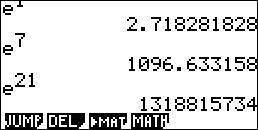
\includegraphics[height=1.75cm]{chap13_expo_casio35}~~~~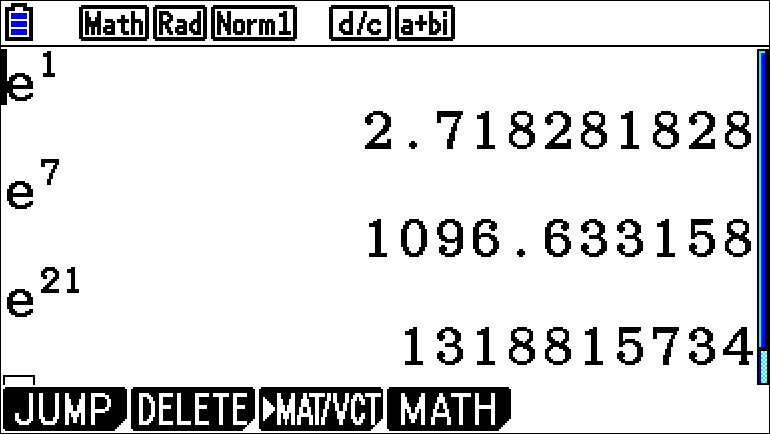
\includegraphics[height=1.75cm]{chap13_expo_casio90}
\end{center}
\end{ccalco}

\section{Compléments}

\subsection{Résolution d'équations et d'inéquations}

\begin{cprop}
Comme la fonction exponentielle est strictement croissante sur $\R$, on a pour tous réels $a$ et $b$ :
\begin{itemize}
	\item $\e^a=\e^b \ssi a=b$ ;
	\item $\e^a \pp \e^b \ssi a \pp b$.
\end{itemize}
\end{cprop}

\begin{cexemple}
Résoudre dans $\R$ les équations suivantes :
\begin{itemize}[leftmargin=*]
	\item $3\e^{-4x+1} - 3\e=0 \ssi \e^{-4x+1}=\e=\e^1 \ssi -4x+1=1 \ssi -4x=0 \ssi x=0$.
	\item $\e^{3x+2} =e^{-4} \ssi 3x+2=-4 \ssi 3x=-6 \ssi x=-2$.
	\item $\e^{x^2}-\e^{9} =0 \ssi \e^{x^2}=\e^9 \ssi x^2=9 \ssi x=\pm3$. 
\end{itemize}
Résoudre dans $\R$ les inéquations suivantes :
\begin{itemize}[leftmargin=*]
	\item $\e^{3x+1} >1 \ssi \e^{3x+1} >\e^0 \ssi 3x+1 > 0 \ssi x > -\tfrac{1}{3}$. 
	\item $\e^{-2x+2} \geqslant \e^{4} \ssi -2x+2 \geqslant 4 \ssi -2x \geqslant 2 \ssi x \leqslant -1$. 
	\item $\e^{x+1}+\e^{-7x+9} <0 \ssi \e^{x+1} < -\e^{-7x+9} <0$ qui est impossible. 
\end{itemize}
\end{cexemple}

\subsection{Fonctions composées}

\begin{cdefi}
Soit $k$ un réel strictement positif. Les fonctions définies sur $\R$ par les expressions $f(t)=\e^{kt}$ et $g(t)=\e^{-kt}$ sont appelées de façon générale \textbf{fonctions exponentielles}.

Elles sont composées d'une fonction \textit{linéaire} suivie de \textit{la} fonction exponentielle.
\end{cdefi}

\begin{cprop}
Soit $k$ un nombre réel strictement positif, et $f$ et $g$ des fonctions exponentielles définie sur $\R$.

$\bullet~~$Si {\red $f(t)=\e^{kt}$}, alors $f'(t)=k \times f(t)=k\e^{kt}$ et $f$ est strictement \textbf{\red croissante} sur $\R$.

$\bullet~~$Si {\blue $g(t)=\e^{-kt}$}, alors $g'(t)=-k \times g(t)=-k\e^{-kt}$ et $g$  est strictement \textbf{\blue décroissante} sur $\R$.

\begin{center}
	\begin{tikzpicture}[x=0.7cm,y=0.7cm,xmin=-3,xmax=3,ymin=-1,ymax=4]
		\axes \fenetre
		\draw[very thick,red,samples=200,domain=3:-3] plot (\x,{exp(0.5*\x)}) node[above right]{$f$} ;
		\foreach \x in {-2,-1,...,2} {
			\draw[thick] (\x,0.1cm) -- (\x,-0.1cm) node[below,scale=0.8] {$\x\strut$};
		}
		
		\foreach \y in {0,1,2,3} {
			\draw[thick] (0.1cm,\y) -- (-0.1cm,\y) node[left,scale=0.8] {$\y\strut$};
		}
		
	\end{tikzpicture}
	\hspace{0.5cm}
	\begin{tikzpicture}[x=0.7cm,y=0.7cm,xmin=-3,xmax=3,ymin=-1,ymax=4]
		\axes \fenetre
		\draw[very thick,blue,samples=200,domain=-3:3] plot (\x,{exp(-0.9*\x)}) node[above left]{$g$} ;
		%\draw (2,0.5) ;
		\foreach \x in {-2,-1,...,2} {
			\draw[thick] (\x,0.1cm) -- (\x,-0.1cm) node[below,scale=0.8] {$\x\strut$};
		}
		
		\foreach \y in {0,1,2,3} {
			\draw[thick] (0.1cm,\y) -- (-0.1cm,\y) node[left,scale=0.8] {$\y\strut$};
		}
		
	\end{tikzpicture}
\end{center}
\end{cprop}

\begin{cdemo}
Les formules de dérivation sont admises, mais pour étudier les variations de la fonction, il suffit d'étudier le signe de la dérivée, sachant que $k>0$, $\e^{kt}>0$ et $\e^{-kt}>0$ (toute image par une exponentielle est toujours strictement positive, même si l'antécédent est négatif).
\end{cdemo}

\begin{crmq}
Il suffit, pour dériver ces fonctions, de les multiplier par le coefficient directeur de la fonction linéaire qui est à l'intérieur de l'exponentielle !
\end{crmq}

\begin{cprop}
On a les formules de dérivation composées suivantes :
%
\begin{itemize}
	\item $\left(\e^{ax+b}\right)^{\prime} = a \times \e^{ax+b}$ ;
	\item si $u$ est dérivable sur $I$, alors $\e^u$ l'est également, et $\left(\e^u\right)^{\prime} = u' \times \e^u$.
\end{itemize}
\end{cprop}

\begin{crmq}
On peut retenir ces formules en disant qu'on fait \og sortir la dérivée \fg{} de ce qui se trouve dans l'exponentielle.
\end{crmq}

\begin{cexemple}[s]
On a, par exemple :
%
\begin{itemize}
	\item $\left(\e^{5t}\right)^{\prime}=5\e^{5t}$ ;
	\item si $f(x)=4\e^{2x}$, alors $f'(x)=4 \times 2 \times \e^{2x}=8\e^{2x}$ ;
	\item si $g(x)=(2x+3)\e^{5x}$, alors $g'(x)=2 \times \e^{5x} + \left(5 \times \e^{5x}\right) \times (2x+3) = (2x+3) \times \big(2 + 5(2x+3)\big) = (10x+17)\e^{5x}$ ;
	\item si $h(x)=10 \e^{x^2-5x+4}$, alors $h'(x)=10 \times \left( (2x-5) \times \e^{x^2-5x+4}  \right) = (20x-50) \e^{x^2-5x+4}$.
\end{itemize}
\end{cexemple}
%
%\begin{chistoire}
%\vspace{-0.22cm}
%\lettrine[findent=.5em,nindent=0pt,lines=3,image,novskip=0pt]{newton}{}La construction de la notion de \textbf{dérivation} (et ses applications) n’a pas été un long fleuve tranquille. L’Europe de la fin du XXII\up{e} siècle a été le théâtre d’un affrontement scientifique entre deux écoles de pensée, d’un côté le monde anglais véhicule les « fluxions » de Newton tandis que le reste de l’Europe porte la pensée de Leibniz. 
%
%Voici comment, dans son ouvrage (1687), Newton exprime sa vision des dérivées :
%
%« Les rapports ultimes dans lesquels les quantités disparaissent ne sont pas réellement des rapports de quantités ultimes, mais les limites vers lesquelles les rapports de quantités, décroissant sans limite, s’approchent toujours, et vers lesquelles ils peuvent s’approcher aussi près qu’on veut. »
%
%\smallskip
%
%\hfill\textit{\tiny Tiré du BARBAZO de 1\up{ère}, 2019}
%\end{chistoire}

\end{document}